\documentclass{oblivoir}
\usepackage{amsthm}
\usepackage{thmtools}


\usepackage{graphicx}

%\usepackage{ansform}
\usepackage{ikps}

\declaretheoremstyle[% spaceabove=6pt,spacebelow=6pt, headfont=\color{MainColorOne}\sffamily\bfseries, notefont=\mdseries, notebraces={[}{]}, bodyfont=\normalfont,
headpunct={},
postheadspace=1em,
%qed=▣,
]{maintheorem}

\declaretheorem[%
name=정의,
style=maintheorem,
numberwithin=section, shaded={%bgcolor=MainColorThree!20,
margin=.5em}]{dfn}
% \begin{dfn}[]
% \end{dfn}

\newtheorem{theorem}{Theorem}[section]
\newtheorem{corollary}{Corollary}[theorem]
%https://www.overleaf.com/learn/latex/Theorems_and_proofs
%http://web.mit.edu/rsi/www/pdfs/theorems.pdf
%https://texfaq.org/FAQ-proof
\declaretheorem[%
name=정리,
style=maintheorem,
numberwithin=section, shaded={%bgcolor=MainColorThree!20,
margin=.5em}]{thm}

%\newcommand{}[][]{}
\setcounter{secnumdepth}{3}
%https://tex.stackexchange.com/questions/130795/how-can-i-number-sections-below-subsection-in-latex


\begin{document}

\tableofcontents


\section{GRAPHS AND SUBGRAPHS}
\subsection{Graphs and simple Graphs}

\begin{dfn}[Graph] 정점과 정점을 잇는 간선들로 이루어진 것을 그래프라한다.
    \begin{itemize}
        \item $V(G)$ :  정점의 집합
        \item $E(G)$ :  간선의 집합
        \item $\psi_G(e_n)$ :  각 간선($e_n$)의 정점의 쌍
        \item $\nu(G)$ :  정점의 갯수 
        \item $\varepsilon(G)$ :  간선의 갯수
    \end{itemize}

    
    그래프를 간선들이 교차하지않게 그릴수 있는 것을 plannar graph라 한다. plannar graph가 아닌 것을 nonplanar graph라한다.
    
    정점이 한개인 그래프를 trivial graph라고 한다. 이외의 모든 그래프는 nontrivial 그래프이다.

    Simple graph : loop가 없고 두 정점쌍에 두개이상의 간선이 존재하지않는 그래프

    incident : 한 간선에 양 정점 근접
    adjacent : 두 간선에 공통된 정점 인접

    
\end{dfn}

\subsection{Graph Isomorphism}

\begin{dfn}[isomophic] 두 그래프 G와 H가  전단사 함수 $\theta : V(G) \longrightarrow V(H)$와 $\phi : E(G) \rightarrow E(H)$이 성립하면 두 그래프는 동형(isomophic)이다.
    또한 다음이 성립한다.
\begin{itemize}
    \item $\psi(e) = us( e \in E(G), u,s \in V(G)) $
    \item $\psi(\phi(e)) = \theta(u)\theta(v)$% $\phi(e)$ %($\phi(e) \in E(H)$)
\end{itemize}
\end{dfn}

\begin{dfn}[a special classes of graphs] 특징에 따른 그래프 이름
    \begin{itemize}
        \item complete graph(완전 그래프) : 모든 정점에 간선이 연결된 그래프 정점의 개수가 $n$일때 $K_n$로 표현한다.
        \item empty graph : 정점이 한개고 간선이 없는 그래프
        \item bipartite graph(이분 그래프) : 정점이 두 집합으로 이루어져 집합 내에는 연결된 간선이 없는 그래프
        \item complete bipartite graph(완전 이분 그래프) : 한 집합의 모든 정점이 각각 반대 집합의 모든 정점에 연결된 그래프 두 정점 집합의 갯수가 각각 $m$과  $n$일때 $K_{m,n}$으로 표현한다.
        \item (1.2.9)k-partite graph : 정점이 적어도하나 포함된 k개의 부분 집합으로 이루어진 그래프이다  한 부분집합 내에 연결된 간선은 존재하지 않고 다른 부분집합의 정점에만 간선이 존재할수있다.
        (원문)a complete k-partite graph is one that is simple and in which each vertex is
        joined to every vertex that is not in the same subset
        \item (1.2.9)complete k-partite graph : k-partite graph의 각 정점이 포함된 부분집합을 제외한 모든 정점에 간선이 연결된 그래프 
        
        (원문)complete k-partite graph is one that is simple and in which each vertex is
        joined to every vertex that is not in the same subset.

        \item (1.2.10)k -cube : 각 정점은 하나의 ordered k-tuple(k-비트 이진수)이고, 두 정점이 1비트만 서로 다를 때 두 정점간에 에지가 있다.
        \item (1.2.11)여 그래프(complement graph) : 모든 정점에 대해서 포함하고 있는 존재하는 간선은 제거, 존재하지않는 간선을 생성해서 만든 그래프 
        $G^{c}$로 표현한다.
        \item (1.2.11)자기 여 그래프 (self-complementary graph) : 여그래프와 자기자신이 동형인 그래프
    \end{itemize}
\end{dfn}

week1

\subsubsection{}
\subsubsection{}
\subsubsection{}
\subsubsection{}
\subsubsection{} %1.2.5
$G \cong H$ , simple

bijection $\theta : V(G) \longrightarrow V(H)$
$ uv \in E(G) \Leftrightarrow  \theta(u)\theta(v) \in E(H)$

정의로 부터 $\psi(e) = us$인 간선 $e$ ($e \in E(G)$)에 대해 대응되는 $\psi(\phi(e)) = \theta(u)\theta(v)$인 $\phi(e)(\phi(e) \in E(H))$가 존재함을 알 수 있다. 
따라서 $ uv \in E(G) \rightarrow \theta(u)\theta(v) \in E(H)$ 성립, 반대의 경우도 마찬가지로 성립한다.

\subsubsection{}
\subsubsection{}
\subsubsection{}
\subsubsection{}%1.2.9

\begin{align}
&{n \choose 2} -  (m(k+1)-n) {k \choose 2} -(n-mk){k+1 \choose 2} \\
&= {n \choose 2} -  m(k+1){k \choose 2}-n{k \choose 2} -(n-mk){k+1 \choose 2} \\
&= {n \choose 2} -  m(k-1){k+1 \choose 2} +n{k \choose 2} -(n-mk){k+1 \choose 2} \\
&= {n \choose 2} + n{k \choose 2} -(n-m){k+1 \choose 2} \\
&= {n \choose 2} + n{k \choose 2} -(n-m){k+1 \choose 2} +(n-1){k+1 \choose 2} - (n-1){k+1 \choose 2}\\
&= {n \choose 2} + n{k \choose 2} - (n-1){k+1 \choose 2} + (m-1){k+1 \choose 2}  \\
&= \dfrac{n^2-n-nk + k^2+k-nk}{2}  + (m-1){k+1 \choose 2} \\
&= \dfrac{(n-k)(n-k-1)}{2}={n-k \choose 2}  + (m-1){k+1 \choose 2}
\end{align}

\subsubsection{}
\subsubsection{}
%1.2.11
(a):
\begin{itemize}
    \item $K_{n}^{c}$ : 간선이 없는 그래프이다.
    \item $K_{n,m}^{c}$ : 두 집합사이의 간선이 없이 두 집합이 각각 완전그래프인 subgraph를 이루고있다.
\end{itemize}
(b): 자기 여 그래프가 되기위해선 일단 동형 이전에 간선의 갯수가 동일해야하는데 여기서 총 생길수있는 간선의 갯수는 $\dfrac{v(v-1)}{2}$가 최댓값이자 그래프의 간선수 + 여그래프의 간선수 입니다. 그래프의 간선수 = 여그래프의 간선수 이므로 $v$나 $v-1$은 적어도 둘 중 하나는(적어도지만 사실 둘다 4의 배수인 경우의 수는 존재하지않습니다) 4의 배수여야합니다 따라서 $v\pmod{4}$는 0 또는 1


\begin{itemize}
\item 추가문제 :

인접성 : 두 그래프가 인접성을 보존할때, $u$와 $v$가 인접하면 $\theta(u)$와  $\theta(v)$가 인접하고 그 역도 성립한다. 

두 그래프 G와 H에 대해서 G의 정점들을 H의 정점들에 일대일로 대응하면서 
인접성을 보존하는 함수 f가 존재하면 두 그래프 G와 H는 동형(isomorphic)이다.

Proof: $E(G)$의 임의의 간선 $e$에 대해 임의의 정점 $u,v$가 인접할때, 인접성이 보존되므로 $\theta(u)$와  $\theta(v)$ 또한 인접한다.
$\theta(u)$와  $\theta(v)$를 잇는 간선을 $e'$이라 할때 $\phi(e) = e'$인 $\phi: E(G) \longrightarrow E(H)$를 정의할 수 있다.
따라서 정의에 의해 $G$와 $H$는 동형이다.
\end{itemize}

week2

\subsection{The Incidence and Adjacency Matrices}
(대충 그래프를 나타내는 표현에 대한 내용)
\subsection{Subgraphs}
\begin{dfn}[subgraph]
    그래프 $H$, $G$가 $ V(H) \subset V(G), E(H) \subset E(G)$, and $\psi_{H}$ is restricton $\psi_{G}$ \protect\footnote{$\psi_{H}$가 제한적으로 $\psi_{G}$이다.} 일때  $H \subseteq G$ 라쓰고 $H$($G$)를 subgraph(supergraph)라 한다.

    \begin{itemize}
        \item $H \subseteq G$,$H\neq G $이면 $ H \subset G$라 표기하고, $H$를  $G$의 proper graph라 한다.
        \item $V(H) = V(G) , H \subseteq G $이면 $H$($G$)를  spaning subgraph(supergraph)라 한다.
        \item spaning subgraph과 동시에 simple graph이면, undelying simple graph라한다.
    \end{itemize}
\end{dfn}
\subsection{Vertex Degrees}
\begin{dfn}[degree(차수)] $d_G(v)$는 정점 $v$에 연결된 간선의 갯수를 나타낸다. 그래프의 정점의 차수의 최솟값을 $\delta(G)$ , 최댓값을 $\Delta(G)$로 표기한다.
    \[
        \sum_{v \in V} d(v) = 2 \varepsilon  
    \]
    k-regular graph(정규그래프) : $d(v) = k \:\forall v \in V$
    $|A|$ : 집합 $A$의 원소의 갯수
\end{dfn}

\begin{theorem}
    \[
        \sum_{v \in V} d(v) = 2\varepsilon  
    \]
\end{theorem}

\begin{proof}
    근접행렬 $M$을 생각해보자 각 열은 정점으로 이루어져있으므로 행의 합은 해당 정점의 차수이다. 따라서 모든 행과 열의 합은 $\sum_{v \in V} d(v)$이며 또한 $2\varepsilon $이다. 예제 1.3.1(a)에 따라서 각 열의 합이 2이다. 
\end{proof}

\begin{corollary}
    어떤 그래프의 차수가 홀수인 정점의 갯수는 짝수이다.
\end{corollary}

\begin{proof}
    차수가 홀수와 짝수인 $V_1$, $V_2$로 정점을 나누었을 때,
    \[
        \sum_{v \in V_1} d(v) + \sum_{v \in V_2} d(v) = \sum_{v \in V} d(v)
    \]
    는 짝수이다. $\sum_{v \in V_2} d(v)$는 짝수이므로 $\sum_{v \in V_1} d(v)$ 또한 짝수이다. 그러므로 $|V_1|$은 짝수이다.
\end{proof}

\subsubsection{}
\subsubsection{} 
%1.5.2
M'는 M의 전치행렬 원표기 $M^{T}$,
$MM'[v_i][v_i] = \sum_{j=1}^n M[v_i][e_j] \cdot M'[e_j][v_i]$

$ M'[e_j][v_i] = M[v_i][e_j] $이며 simple graph일때 각 값은 0 또는 1이기 때문에 결과적으로 대각선의 값은 해당 정점의 차수가 된다.

$A$ 행렬에서 $A[v_i][v_j] = A[v_j][v_i]$ 

$d(i) = \sum_{j=1}^n A[v_i][v_j] = \sum_{j=1}^n A[v_j][v_i]$이다.
마찬가지로 simple graph에서 $A[v_i][v_j]$은 무조건 0 또는 1을 가지므로 $A[v_i][v_j] \cdot A[v_j][v_i] = A[v_i][v_j]$이다.

$A^2$에서 $A^2[v_i][v_i] = \sum_{j=1}^n A[v_i][v_j] \cdot A[v_j][v_i]= \sum_{j=1}^n A[v_i][v_j] = d(i)$

\subsubsection{} 
% 1.5.3

k-regular bipartite graph의 bipartition($X$,$Y$)이 $|X|\neq |Y|$라 하자. $d(v)=|Y|,\: d(u)=|X|(v \in X, u \in Y )$ $d(v) \neq d(u)$ 이는 k-regular graph의 조건에 모순

\subsubsection{} 
% 1.5.4

두명 이상의 사람이 있는 그룹에서 그룹 내 친구의 수(그룹 내부의 사람으로 제한)가 같은 사람이 반드시 두명이 있음을 보여라

사람이 n명일때 친구의 수는 최대 n-1명이기때문에 비둘기집의 원리에 의해 친구 수가 같은 사람이 무조건 두명이 존재한다.

각각의 사람을 정점, 친구관계를 간선으로 나타낸다면은 해당 그룹은 simple graph로 볼수있으며 친구의 수는 각 정점의 차수가 된다.

따라서 해당 문제는 simple graph일때 반드시 두 정점의 차수가 같음을 보이는 것과 같다. 
\subsubsection{} 
% 1.5.5
만약 $G$가 정점 $v_1, v_2, ... , v_n$을 가질때 $(d(v_1), d(v_2), ... , d(v_n))$ 을 그래프 $G$의 차수 수열(degrees sequence)라 부른다.

음이 아닌 정수들의 시퀀스 $(d_1, d_2, ... , d_n)$가 어떤 그래프의 차수 시퀀스임이 $\sum_{i=1}^n d_i$가 짝수임과 필요충분 조건임을 보여라.

그래프의 차수의 합은 $2\varepsilon$임이  $Theorem1.1$에 이미 증명되어 있다. 따라서 차수 수열의 합은 짝수이며 반대의 경우도 성립한다.


If G has vertices $(v_1, v_2, ... , v_n)$ the sequence $(d(v_l), d(v_2), ... , d(v_n))$ is called a degree sequence of G. 
Show that a sequence $(d_1, d_2, ... , d_n)$ of non-negative integers is a degree sequence of some n
graph if and only if $\sum_{i=1}^n d_i$ is even

\subsubsection{} 
% 1.5.6 
    A sequence $d = (d_1, d_2 , ... , d_n)$ is graphic if there is a simple graph with degree sequence d. Show that

(a) (7,6,5,4,3,3,2) : 정점이 총 7갠데 첫번째 정점의 간선이 7개인것은 simple graph의 조건을 충족하지 못한다.
(6,6,5,4,3,3,1) : 총 7개의 정점중 자신을 제외한 모든 정점에 간선을 잇는 차수가 6인 정점이 2개이지만 차수가 1인 정점이 있으므로  simple graph임이 모순이다.

(b) if $d$ is graphic and $d_1 \le d_2 \le ... \le d_n$, then $\sum_{i=1}^{n} d_i$ is even and $\sum_{i=l}^{k} d_i \le k(k -1)+\sum_{i=k+1}^{n}\min(k, d_i)$ for $1 \le k \le n$

그래프가 심플그래프일때 차수 수열이 $d_1 \le d_2 \le ... \le d_n$이면,  $\sum_{i=1}^{n} d_i$ 짝수인것과 다음이 성립함을 보이시오
$\sum_{i=1}^{k} d_i \le k(k -1)+\sum_{i=k+1}^{n}\min(k, d_i)$ for $1 \le k \le n$

d는 차수수열이므로 d의 합은 $2\varepsilon$이다.
\subsubsection{} 
%
\subsubsection{} 
%
\subsubsection{} 
%
\subsubsection{} 
%1.5.10

The edge graph of a graph G is the graph with vertex set E(G) in
which two vertices are joined if and only if they are adjacent edges in G. 

Show that, if G is simple
(a) the edge graph of G has e(G) vertices and L (d2 (V)) edges; vEVlG) .
(b) the edge graph of Ks is isomorphic to the complement of the graph featured in exercise 1.2.6.

그래프 G의 엣지 그래프는 꼭지점 집합 E (G)가있는 그래프로 두 개의 꼭지점이 G의 인접 엣지 인 경우에만 결합됩니다.

\subsection{Paths and Connection}
\begin{dfn}[walk]순차적으로 이어지는 정점, 간선의 연결을 walk라한다. $v_{0}e_{1}v_{1}e_{2}v_{2} ... e_{k}v_{k}$인 walk를 $v_0$ to $v_k$ 또는 ($v_0$, $v_k$)-walk라 한다.
    \begin{itemize}
        \item 지나는 간선을 한번씩만 쓴 walk를 trail이라한다.
        \item simple graph $G$의 모든 간선을 지나는 trail의 길이는 $\varepsilon (W)$이다.
        \item 지나는 정점을 한번씩만 쓴 walk를 path라 한다
        \item 그래프 G가 두 정점 u,v의  (u,v)-path가 존재할때, connected graph라한다.
        \item 그래프의 정점을 쪼갠 부분 그래프들이 모두 각각의 연결된 그래프일때, 부분 그래프들을 그래프 G의 component라 한다.
        \item 그래프 G의 componet의 수를 $\omega(G)$라 쓴다.
    \end{itemize}
\end{dfn}
\subsubsection{} 
% 1.6.1 

($u$,$v$)-walk사이에 사이클이 존재 할 경우 겹치는 정점을 중복사용하지않는 walk를 짤수있다 따라서 ($u$,$v$)-path가 존재한다.
\subsubsection{} 
%1.6.2
????

\subsubsection{} 
%1.6.3
한 정점을 패스의 시작정점으로 잡았을때 $\delta \le k$ 이기때문에  lenth가 $k$인 path를 만들기위해 서로 다른 $k$개의 연결된 정점을 선택해 path를 생성할수있다.
\subsubsection{} 
% 1.6.4
????
\subsubsection{} 
%1.6.5
(a) : 최대한 적은 정점에 많은 간선을 사용한 그래프를 세팅하기위해,  정점 하나를 제외한 $\varepsilon-1$개의 정점으로 ${\varepsilon-1 \choose 2}$개의 엣지를 사용한 완전 그래프를 만들면 완전 그래프내의 정점들로는 더이상 간선을 연결 할 수 없기 때문에 조건의 그래프는 무조건 connected가 된다.

(b) : 정점 하나를 제외한 $\varepsilon-1$개의 정점으로 ${\varepsilon-1 \choose 2}$개의 엣지를 사용해 완전 그래프를 만들면 정점하나는 연결되어 있지않으므로 disconnected그래프이다.
\subsubsection{} 
%
\subsubsection{} 
%
\subsubsection{} 
% 1.6.8

(a)간선 e가 빠짐으로서 하나였던 component가 두개의 component가 될 요지가 있다. 따라서 $\omega(G) \le \omega(G-e) \le \omega(G)+1 $가 성립한다.

(b) inequality: 부등식
반례: $V(G) = { v_1, v_2, v_3} ,\: E(G) = { e_1 , e_2} ,\: \psi_H(e_1) = v_1v_1 ,\psi_H(e_2) = v_2v_3  $
$v_1$과 $v_2v_3$가 각각 연결되어있는 $\omega(G) = 2$인 그래프이다$v_1$을 제거할때 component가 하나 사라지므로 주어진 부등식을 만족하지 못한다.
\subsubsection{} 
%1.6.9
\subsubsection{} 
% 1.6.10
\subsubsection{} 
% 1.6.11
\subsubsection{} 
% 1.6.12
\subsubsection{} 
% 1.6.13

\subsubsection{} 
% 1.6.14
$uv, uw, uw \in E $이면 $G$는 complete가 되기때문에 $uw \notin E$

\subsection{Cycles}

\begin{dfn}[cycle]
walk가 양의 길이이고 시작점과 끝점이 같을때 닫혀있다(closed)고 한다. 

닫힌 트레일을 cycle이라고한다.
\end{dfn}

\begin{theorem}
    그래프가 이분그래프인것과 홀수개의 사이클을 가지지 않는것은 필요충분조건이다.
\end{theorem}
\begin{proof}
    
\end{proof}
\subsubsection{} 
% 1.7.1
\subsubsection{} 
%1.7.2
simple graph가 아닌경우
        루프를 포함하는경우 $v_0v_0$는 정의에 의해 사이클이다.
            임의의 정점$v_0, v_1$에 간선이 2개이상인경우            $v_0v_1v_0$사이클을 이룬다
        
    simple graph인경우
        정점의 개수가 k인 그래프를 생각하자. 이때 $v_0v_1v_2 ... v_i$인 서로 다른 정점만 최대한 이어진 연결을 생각해볼때 $v_0$과 $v_i$의 차수는 명제의 조건에의해서 무조건 $0 \le j \le k$인 정점 $v_j$에 연결이 되어있어야한다. 따라서 $v_{j}v_{j+1} ... v_k$인 사이클을 이룬다.
\subsubsection{} 
% 1.7.4
\subsubsection{} 
% 1.7.5
\subsubsection{} 
% 1.7.6

week 3
\subsection{The Shortest Path Problem }
(대충 Dijkstra's Algorithm에 대한 내용)
\subsubsection{} 
%
\subsubsection{} 
%
\subsubsection{} 
%
\subsubsection{} 
%
\subsubsection{} 
% 1.8.5

가능한 모든 경우의 수를 센다. 이때 양방향이아닌 한방향 간선은 사이클을 형성하므로 최적의 경로로서 제외해도 문제없다.

\begin{enumerate}
    \item 시작 (8,0,0) $\rightarrow$ 2,3
    \item (3,5,0) $\rightarrow$ 1,4,5
    \item (5,0,3) $\rightarrow$ 1,4,6
    \item (0,5,3) $\rightarrow$ 2,3,5
    \item (3,2,3) $\rightarrow$ 2,4,7
    \item (5,3,0) $\rightarrow$ 3, 8
    \item (6,2,0) $\rightarrow$ 5,9
    \item (2,3,3) $\rightarrow$ 6
    \item (6,0,2) $\rightarrow$ 7,10
    \item (1,5,2) $\rightarrow$ 9,11
    \item (1,4,3) $\rightarrow$ 10,12
    \item 끝 (4,4,0) $\rightarrow$ 11,13,14
    \item (4,1,3) $\rightarrow$ 12
    \item (1,4,3) $\rightarrow$ 12
\end{enumerate} 
1 $\rightarrow$ 2 $\rightarrow$ 5 $\rightarrow$ 7 $\rightarrow$ 9 $\rightarrow$ 10 $\rightarrow$ 11 $\rightarrow$ 12
\subsubsection{} 
% 1.8.6

\subsection{Sperner's Lemma.}
2차원 평면상의 삼각형$T$ 에 대해서 이를 작은 삼각형으로 쪼갤때 교차하는 
삼각형이 꼭지점 또는 전체면을 공통으로 가질때 이 삼각형을 쪼갠것을 단순하다(be simplicial)라고 한다.

그다음 단순한 삼각형의 쪼갬에 대해서 쪼개진 각 정점에 대해서 다음이 성립할때, 0,1,2 세개의 분류(labelling)가 
적절(be proper)하다고 한다.


\begin{figure}[h!]
    \centering
    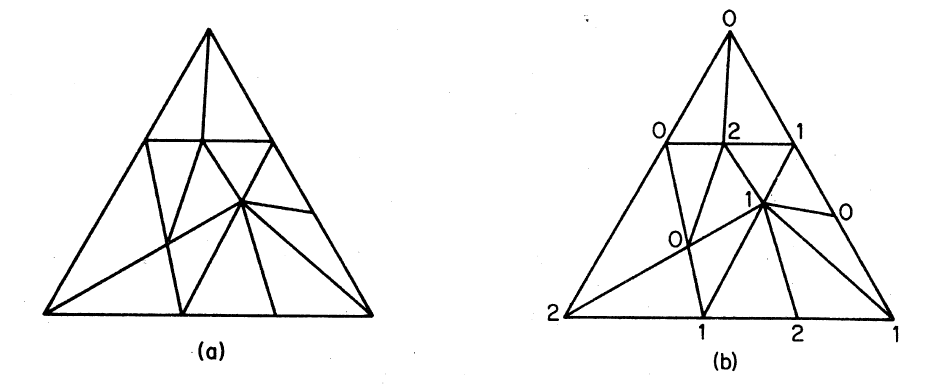
\includegraphics[scale=0.5]{simp.png}
    \caption{(a) Asimplicial subdivision of a triangle (b) a proper labelling of the    subdivision}
\end{figure}



\begin{itemize}
    \item T의 세개의 정점에는 0,1,2가 하나씩 붙는다.
    \item 그리고 T의 정점 사이의 정점에는 양 끝 T의 정점의 두 값만 값이 붙을 수 있다.
\end{itemize}
각 정점을 0,1,2로 가지는 삼각형을 구별된 삼각형이라한다.

\begin{theorem}[Sperner's lemma]
    적절히 분류되고(properly labelled) 단순하게(simplicial) 삼각형을 쪼갠것은 내부에 홀수개의 구별된 삼각형을 가진다.
\end{theorem}

\begin{proof}
    $T$를 $T_0$라 하자. 그다음 $T_1,T_2,...,T_n$을 쪼개진 삼각형들이라고 하자. 
    0과 1로 각각 분류된 $T_i$와 $T_j$가 공통 간선일때 $v_i$,$v_j$에 간선이 존재하는
    정점 집합 $\{v_0,v_1, ... ,v_n \}$을 정의하자.(이 정점은 T에 대응할수있다.)
    
    이 그래프에서 $v_0$는 명백하게 차수가 홀수값을 가진다.(1.9.1) 
    따라서 $v_1,v_2,...,v_n$중에 홀수개가 홀수값 차수를 가지게 된다.
    삼각형이라서 이 홀수개의 차수를 가지는 정점들이 차수값이 오직 1만을 가짐을 알 수 있다.
    $v_i$의 차수가 1임은 $T_i $가 구별된 삼각형인 경우만이다.
\end{proof}

\subsubsection{}
%191




week 4
\section{Tree}
\subsection{Trees}

\begin{dfn}[tree] connected acyclic graph

    acyclic graph : 사이클이 없는 그래프
\end{dfn}

\subsubsection{} 
%
\subsubsection{} 
%
\subsubsection{} 
%
\subsubsection{} 
%
\subsubsection{} 
%  2.1.5
Let 0 be a graph with v-I edges. Show that the following three statements are equivalent: 
(a) G is connected;
(b) G is acyclic;
(c) G is a tree.

연결된 acyclic graph는 정의에 의해 tree임이 자명하므로 간선의 개수가 $\nu -1$  일때, acyclic graph일때 connected한것과 connected graph일때 acyclic 그래프임이 필요충분조건임을 보이는 것으로 충분하다.

acyclic $\rightarrow$ connected graph

acyclic그래프가 connected graph가 아니라고 가정해보자.

그러면 각 component는 connected graph이므로 트리이다.
각 component의 간선의 갯수의 합은 $v(G_1)-1 + v(G_2)-1 + ... + v(G_n)-1 \neq v(G)-1 $
따라서 가정에 모순 다음 명제가 성립한다.

connected graph $\rightarrow$ acyclic

acyclic graph가 아니라고 하자 cycle이 형성된곳의 간선을 하나씩 제거해서 acyclic 그래프가 되도록 만들면 트리가 된다.
$\nu-1-n \neq \nu -1 $ 가정에 모순이라 다음 명제가 성립한다.
\subsubsection{} 
%
\subsubsection{} 
%
\subsubsection{} 
% 2.1.8
A centre of G is a vertex u such that max d(u, v) is as small as possible.
Show that a tree has either exactly one centre or two,
adj acent, centres.


G의 중심은 최대 d(u, v)가 가능한 한 작은 꼭지점 u이다.

트리 하나가 정확히 하나의 중심 또는 두 개의 인접한 중심을 가지고 있음을 보여라

week5

\begin{dfn}[spanning tree]
    그래프 $G$의 트리인 spanning subgraph를 $G$의 신장 트리(spaning tree)라고 부른다.
\end{dfn}

\begin{corollary}
    $2.4.1$ 모든 연결된 그래프는 스패닝 트리를 가진다.
\end{corollary}

\begin{proof}
    그래프 $G$가 connected graph이면 $G$의 cennected spanning subgraph가 존재한다.
    그래프 $H$를 $G$의 최소한의 connected spanning subgraph라 하자.
    이때 $H$가 acyclic가 아니라고 가정 해보자.
    그래프 $H$가 사이클이 존재하는 경우,간선 사이클 경로의 임의의 인접한 정점 $u, v$를 잡았을때 $u, v$의 간선을 제거해도 $u, v$는 여전이 연결되어있다. 이는 최소한의 connected spanning subgraph라는 것에 모순이다. 
    따라서 그래프 $H$는 connected spaning graph이며 acyclic함으로 스패닝 트리이다.
\end{proof}

\begin{theorem}
    $T$가 연결된 그래프 $G$의 스패닝 트리라고 하고 $e$를 $T$에 속하지 않은 $G$의 에지라고 하자. 그러면 $T + e$는 유일한 사이클을 가진다.
\end{theorem}
\begin{proof}
    $\psi_G(e) = xy$라 할때, 유일한 사이클이아닌 두 개 이상의 사이클이 생성될 경우  e의 에지 추가하기전의 $x, y$ 유일한 경로가아닌 두개이상의 경로가 있다는 것을 의미하는데 트리는 유일한 경로임이 이미 증명되었으므로 유일한 사이클을 가진다.
\end{proof}
\subsection{Cut Edges and Bonds}

\subsection{Cut Vertices}

\subsection{Cayley's Formula}
\begin{dfn}[contract]
    그래프 $G$의 한 에지$e$를 수축한다는 것은 에지 $e$를 그래프에서 삭제하고 양 끝점을 하나의 정점으로 합치는 것이다. 그 결과 만들어지는 그래프를 $G \cdot e$로 표시한다.
    \begin{itemize}
        \item $\nu(G \cdot e) = \nu(G \cdot e) - 1$
        \item $\varepsilon(G \cdot e) = \varepsilon(G \cdot e)-1$
        \item $\omega(G \cdot e) = \omega(G)$
        \item  $T$가 트리이면 $T \cdot e$도 트리이다.
        \item 그래프 G의 스패닝 트리의 개수를 $\tau(G)$로 표시한다.
    \end{itemize}
\end{dfn}

\begin{theorem}
    2.8 그래프 $G$의 임의의 에지 $e$에 대해서 $\tau(G) =\tau(G-e) + \tau(G \cdot e)$이 성립한다.
\end{theorem}

\begin{proof}
    그래프 $G$에서 에지$e$를 포함하지 않는 스패닝 트리는 $G-e$의 스패닝 트리 또한 된다.
    따라서 $\tau(G-e)$는 그래프 $G$에서 에지 $e$를 포함하지 않는 스패닝 트리의 개수와 같다.
    에지 $e$를 포함하는 $G$의 임의의 스패닝 트리 $T$는 $G \cdot e$의 스패닝 트리 $T \cdot e$에 일대일 대응한다.(추가적인 논리 필요) 따라서 $\tau(G \cdot e)$는 $G$에서 에지 $e$를 포함하는 스패닝 트리의 개수이다. 따라서 정리가 성립한다.
\end{proof}


Fortunately, and rather surprisingly, there is a closed formula for T(G) which expresses T(G) as a determinant; 
we shall present this result in chapter 12.


\begin{theorem}
    $Cayley's folmula$ : $\tau(K_n)= n^{n-2}$
\end{theorem}

\begin{proof}
    $K_n$의 정점 집합을 $N = \{1,2, ...,n\}$라 놓자.
    그러면 $n^{n-2}$는  $N$으로부터 길이가 $n-2$인 수열\footnote{$Pr\ddot{u}fer \: sequences$라 한다.}을 만드는 수로 볼 수 있다.
    따라서 이 수열이 $K_n$의 spanning tree와 1:1대응을 하는걸로 이 증명이 완성된다.
    $K_n$의 spanning tree $T$에 대해서 특정 수열 ${t_1, t_2, ... , t_{n-2}}$과 연관지으려 한다.
    $N$을 정렬된 셋이라 가정하고, $s_1$은 $T$의 차수가 1인 첫번째 정점이라하자. $s_1$은 $t_1$과 인접한 정점이다.
    그다음에 $s_1$를 $T$에서 제거하자 그다음 $T-s_1$에 차수가 1인 정점 한개를 $s_2$라 하자 이 짓거리를 $t_{n-2}$가 지워져 두 정점이 남을때 까지 반복한다. 총 반복은 $n-2$번 반복한다. 따라서 spanning tree가 수열에 대응함을 보였다.
    수열이 spanning tree에 대응함을 보이자.
    sequence P에 없는 1에서 n중 가장 작은 숫자를 찾아 P의 첫번째 숫자에 연결한다.
    그 후 P의 첫번째 숫자를 제거한다.
    P가 존재하지않을 때 까지 반복한다. 마지막 연결되는 숫자는 n이다.
    이렇게 함으로써 수열이 트리에 대응됨을 보일수있다.
    수열의 갯수가 $n^{n-2}$개 이므로 트리의 개수도 $n^{n-2}$개이다.
\end{proof}



\section{Connectivity}

\subsection{Connectivity}

\begin{dfn}[Connectivity] 
    Connectivity
    \begin{itemize}
        \item A vertex cut : $G-V'$가 연결되지않은 그래프인 $V$의 부분 집합 $V'$를 정점 절단(A vertex cut) 이라고한다.
        \item k-vertex cut : k개의 원소를 가진 정점 절단. 완전 그래프(complete graph)는 정점 절단을 가지지 않는다.
        \item 스패닝 서브 그래프로서 완전 그래프를 가지는 그래프는 정점 절단을 가지지 않는다.
        \item  connectivity $\kappa(G)$ : 그래프 $G$가 가지는 $k-vertex cut$의 최소값 $k$를 $\kappa(G)$라고 한다.그래프 $G$가 trivial이거나 연결되지않은 그래프일때 $\kappa(G) = 0$이다.
        \item $k-connected$ :  $\kappa(G) \ge k$일때 그래프 $G$는 $k-connected$이다. 
        \item 모든 nontrivial connected graph는 $1-connected$이다.
    \end{itemize}
\end{dfn}

\begin{dfn}[Edge connectivity]
    Edge connectivity 
    \begin{itemize}
        \item k-edge cut : k개의 원소를 가지는 간선 절단(edge cut).
        \item Edge connectivity $\kappa'(G)$ : nontrivial 그래프 $G$의 k-edge cut $E'$ $G-E'$는 연결되어있지않다. $k-edge cut$를 가지는 $G$의 최소한의 $k$를 $\kappa'(G)$라 표현한다. $G$가 trivial이거나 연결되지않은 그래프 일때, $\kappa'(G) = 0$이다.
        \item $\kappa(G) \ge k$일때 $G$는 k-edge-connected이다.
        \item 그래프 $G$가 연결된 그래프일때  $\kappa'(G)= 1$이고 모든 nontrivial connected 그래프는 1-edge-connected이다.
    \end{itemize}
\end{dfn}


\begin{theorem}
    
\end{theorem}

\subsubsection{}
%3.1.1
(a) Show that if G is k-edge-connected, with $k >0$, and if E' is a set
of $k$. edges of G, then $w(G - E') < 2$

$\omega(G) = 1$

case 1) $k'(G) > k  \rightarrow \omega(G-E') = 1$

case 2) $k'(G) = k  \rightarrow \omega(G-E') = 2$

$ \therefore \omega(G-E') \le 2$


(b) .For $k > 0$, find a k -connected graph G and a set V' of kvertices
of G such that $\omega(G - V') > 2.$

모래시계모양에 가운데 정점에 추가 한 간선에 다른 한 정점이 이어진 모양 

\subsubsection{}
%3.1.2
Show that if G -is k-edge-connected,.then $\epsilon > kv/2.$

Theoream 3.1에 의해 $k \le \delta$ 따라서 $k \times v \le 2\epsilon$

\subsubsection{}
%3.1.3
(a)  : 

case 1) $\delta = v - 1$ 

csae 2) $\delta = v - 2$ 

(b) : 모래시계

\subsubsection{}
%3.1.4
(b) : 모래시계 가운데 정점이 나뉘어져 가운데 간선이 하나 있는경우


\subsubsection{}





\subsection{BLOCKS}

\begin{dfn}[Blocks]
    Block : 절단 정점들이 존재 하지않는 연결된 그래프를 block이라한다.
    적어도 세개 이상의 정점을 가진 모든 블록은 2-connected이다.
    그래프의 블록은 최대로 블록의 성질을 가질수있는 상태이다.(대충 블록이 또 블록으로 쪼개지는 경우는 생각 안한다는것.)
\end{dfn}

\begin{theorem}
    
\end{theorem}






\section{상세 분석}

\subsection{최악의 케이스 분석 }


실제 재귀함수를 일반화 식은 다음이 된다.

$$T(n) = \max_{0 \le q \le n-1}(T(q) + T(n-q-1)) + \Theta(n)$$

이때 $T(n)$이 $\Theta(n^2)$임을 보이면된다.
치환법을 이용해서 이 점화식을 풀수있다.
$T(n) \le c_1n^2$이라 가정하자. 그러면

$$T(n) \le \max_{0 \le q \le n-1}(c_1q^2 + c_1(n-q-1)^2) + \Theta(n)$$

이 성립한다. 

$0 \le q \le n-1$인 $c_1q^2 + c_1(n-q-1)^2$에 대해서 

$f(q) = c_1q^2 + c_1(n-q-1)^2$ 이라하고 $f'(q) = 2c_1q - 2c_1(n-q-1)$이므로 $q=\dfrac{n-1}{2}$일때 극솟값을 가진다. 이 극솟값은 $q$의 존재 범위에 포함되고 따라서 이차함수의 특성에 따라 양 끝점이 최댓값이 될수있는 후보가된다. $q=0$일때와 $q=n-1$일때 극댓값을 가지는데 이때의 두 함숫값은 같아서 둘중 어느값을 택해도 최댓값이 된다.

\begin{align*}
    T(n) & \le c_1(n-1)^2 + \Theta(n) \\
    & \le c_1n^2 - c(2n-1) + \Theta(n) \\
    & \le c_1n^2    
\end{align*}


이때 $\Theta(n) = dn$에서 $ c_1 > d $인 상수 $c_1$을 가지게 함으로 써 결과적으로 $T(n)$이 $c_1n^2$보다 작거나 같음을 보일수있다. 반대로 $c_2n^2 \le T(n)$임을 가정하고  $ c_2 < d $인 상수를 잡음으로 $T(n)$이 $c_2n^2$보다 크거나 같음을 보일수있다. 따라서 $T(n) = \Theta(n^2)$를 얻을 수 있다.


\subsection{기대 수행 시간}

1 부터 모든 n에 대해서 모든 비용의 평균.

%$\dfrac{\sum_{i=1}^{n}E[X_i]}{n}$

\begin{align*}
    E[X] &= E\left[ \sum_{i=1}^{n}X_i \right] \\
    &= \sum_{i=1}^{n}E\left[X_i \right]   
\end{align*}
 
시간복잡도를 분석하기위해서 다음의 보조정리를 이용한다.


% Let X be the number of comparisons performed in line 4 of PARTITION over the entire execution of QUICKSORT on an n-element array. 

% Then the running time of QUICKSORT is O(n + X)
\begin{lemma}
    X가 길이가 n인 배열에서 QUICKSORT의 전체 실행에 대해서 PARTITION의 4행에서 수행된 비교문의 실행 수라고 가정하면 QUICKSORT의 실행시간은 O(N+X)이다.    
\end{lemma}


% By the discussion above, the algorithm makes at most n calls to PARTITION, each of which does a constant amount of work and then executes the for loop some number of times. 
% Each iteration of the for loop executes line 4.

%  PARTITION에 대한 모든 호출에서 수행 된 비교의 총 수인 X를 계산하는 것이다.

% PARTITION에 대한 각 호출에서 얼마나 많은 비교가 이루어 졌는지 분석하려고 시도하지 않습니다.

%  오히려 총 비교 수에 대한 전반적인 경계를 유도합니다.

\begin{proof}
    알고리즘은 PARTITION을 최대 n 회 호출한다. 각 호출은 for 루프를 실행하는데, for 루프의 각 반복은 4행 비교문을 실행한다.    
\end{proof}

따라서 모든 호출에 대해서 총 비교수 X를 구하는 문제로 바뀌는데 각 호출에 대한 비교를 분석하지않고 총 비교수를 계산한다.
그렇게 하기 위해 배열 $A = \{z_1 , z_2, ... , z_n\}$의 각 요소가 내림차순으로 정렬되어있다고 생각한다. 또한 집합 $Z_{ij} = \{z_i, z_{i+1}, ..., z_j\}$라 정의한다. 여기서 $z_i$와 $z_j$는 최대 한번 비교된다. 이유는 PARTITION에서 비교를 하는 경우는 하나의 원소가 pivot으로 선택 되었을 때인데, 이후에 이 pivot은 절대로 다른 원소와 비교하지 않는다.
따라서
%indicator random variables
$X_{ij} = I\{ z_i$가 $z_j$와 비교한다 $\}$

$ X = \sum_{i=1}^{n-1}\sum_{j=i+1}^{n} X_{ij}$

\begin{align*}
    E[x] &= E \left[ \sum_{i=1}^{n-1}\sum_{j=i+1}^{n} X_{ij} \right] \\
    &= \sum_{i=1}^{n-1}\sum_{j=i+1}^{n} E\left[X_{ij} \right] \\
    &= \sum_{i=1}^{n-1}\sum_{j=i+1}^{n}Pr\{ z_i \mbox{가} z_j\mbox{와 비교한다} \} 
\end{align*}    
    
\begin{align*}
    Pr\{ z_i \mbox{가} z_j\mbox{와 비교한다} 
    &= Pr\{ Z_{ij}\mbox{에서} z_i \mbox{또는} z_j\mbox{가 첫번째로 선택된다.}\}\\
    &= Pr\{ Z_{ij} \mbox{에서} z_i \mbox{가 첫번째로 선택된다}.\} + Pr\{ Z_{ij}\mbox{에서} z_j \mbox{가 첫번째로 선택된다.}\} \\
    &= \dfrac{1}{j-i+1} + \dfrac{1}{j-i+1} \\
    &= \dfrac{2}{j-i+1}    
\end{align*}
    

$$E[X] =  \sum_{i=1}^{n-1}\sum_{j=i+1}^{n} \dfrac{2}{j-i+1}$$

이는 $j-i$을 $k$로 치환해서 상한을 얻을 수 있다.

\begin{align*}
    E[X] & = \sum_{i=1}^{n-1}\sum_{j=i+1}^{n} \dfrac{2}{j-i+1}\\
    & =  \sum_{i=1}^{n-1}\sum_{k = 1}^{n-i} \dfrac{2}{k+1} \\
    & \le \sum_{i=1}^{n-1}\sum_{k = 1}^{n} \dfrac{2}{k} \\
    & \le \sum_{i=1}^{n-1} c\lg n \\
    & \le c n \lg n    
\end{align*}


$$E[X]= O(n \lg n)$$

하한은 다음과 같이 직접구한다.
\begin{align*}    
E[X] &= \sum_{i=1}^{n-1}\sum_{k = 1}^{n-i} \dfrac{2}{k+1} \\
& = \sum_{k = 1}^{n-1} \dfrac{2}{k+1} + \sum_{k = 1}^{n-2} \dfrac{2}{k+1} + \cdots + \sum_{k = 1}^{1} \dfrac{2}{k+1}\\
& = (n-1)\dfrac{2}{1+1} + (n-2)\dfrac{2}{2+1} + \cdots +1 \times \dfrac{2}{(n-1)+1}\\
& = \sum_{k=1}^{n-1} \dfrac{2}{k+1} \times (n-k)\\
& = \sum_{k=1}^{n-1} \left( \dfrac{2n}{k+1} -\dfrac{2k}{k+1}\right)\\
& = 2n \sum_{k=1}^{n-1} \dfrac{1}{k+1} - 2\sum_{k=1}^{n-1} \dfrac{k}{k+1}\\
& \ge 2nc\lg n - 2(n-1) \left(\because -\sum_{k=1}^{n-1} \dfrac{k}{k+1} \ge -\sum_{k=1}^{n-1}\left( \dfrac{k}{k+1}+\dfrac{1}{k+1}  \right)\right)\\
& \ge \Omega(n\lg n) 
\end{align*}

따라서 $$\Theta(n\lg n)$$
%%%%%%%%%%%%%%%%%%%%%%%%%%%%%%%%%%%%%%%%%%%%%
\subsection{Hoare's Partition VS Lomuto's Partition}

\textbf{Lomuto’s Partition Scheme}
\begin{lstlisting}[style = CStyle]
PARTITION(A ,p ,r)
    x= A[r] //pivot
    i = p-1
    for j = p to r-1
        if A[j]<= x
            i = i + 1
            exchange A[i] with A[j]
    exchange A[i+1] with A[r]
    return i + 1
\end{lstlisting}


\textbf{Hoare's partition scheme}

\begin{lstlisting}[style = CStyle]
PARTITION(A ,p ,r)
    x= A[r] //pivot
    i = p
    j = r
    while TRUE
        repeat
            j = j - 1
        until A[j] <= x
        repeat
            i = i + 1
        until A[i] >= x
        if i < j
            exchange  A[i] with A[j]
        else return j
\end{lstlisting}


다음 사이트의 답변을 번역했습니다 \href{https://cs.stackexchange.com/questions/11458/quicksort-partitioning-hoare-vs-lomuto}{stackexchange}\\

이해하기 편하고 간편한 알고리즘을 따질때 Lomuto’s Partition이 간편하다. 그렇기에 우리들이 알고리즘을 이렇게 기억하고 있는것일 것이다. 성능적인 측면만 따지면 다음을 비교해 볼 수 있다.

\subsubsection{비교 횟수}
모든 요소가 피봇가 비교하기 때문에 둘다 n-1번 비교한다.

\subsubsection{스왑 횟수}
Lomuto's Partition의 경우 $1 <= x <= n$인 pivot값 $x$에 대해서 스왑은 정확히 $x-1$번 수행한다.
$$\dfrac{1}{n} \sum_{x=1}^{n}(x-1) = \dfrac{n-1}{2}$$

Hoare's Partition의 경우 i는 피봇값보다 큰값 j는 피봇보다 작은 값에 대해서 스왑을 실행한다. 이 스왑을 수행하는 i의 수와 j의 수는 언제나 같은데 (당연히 쌍으로 교환하니까) 이 쌍의 수는 결과적으로  초기하 분포\footnote{학교에서 통계학을 안들어서 저도 잘 모릅니다 ㅠㅠ}를 따른다 따라서 
쌍수는 $\dfrac{(n-x)(x-1)}{n-1}$이 된다.

$$\dfrac{1}{n} \sum_{x=1}^{n} \dfrac{(n-x)(x-1)}{n-1} = \dfrac{n-2}{6}$$



\subsubsection{정렬이 이미 되어있는경우}
Hoare's Partition은 스왑을 실행하지않는다 그러나 Lomuto’s Partition은 $n/2$만큼의 스왑을 수행한다.

\subsubsection{모든 배열이 같은 값으로 설정 되어있을때}

Hoare's Partition는 무한루프에 빠진다. Lomuto’s Partition인 경우 모든 단일 요소에 대해서 스왑을 실행하며 i = n 이 되어 최악의 파티션 또한 가지게되어 수행시간은 $\Theta(n^2)$이 된다.

Hoare's Partition은 실질적인 측면에서볼때 활용도가 \textbf{매우매우매우매우매우매우매우매우매우} 떨어진다. 버그를 내기 매우 쉬운 알고리즘이고 코드 가독성 또한 매우 떨어진다 또한 결정적으로 중복값의 처리가 안되며 이를 고칠시에 결국 성능이 Lomuto’s Partition보다 느리게 된다.\footnote{
참고 : \href{https://stackoverflow.com/questions/7198121/quicksort-and-hoare-partition}{hoare}}

다음의 실제 테스트 결과를 봐도 알 수 있다.\footnote{사진의 출처인데
\href{http://rohitja.in/lomuto-hoare-partitioning.html}{Hoare, Lomuto testing} 테스트 케이스가 상당히 아쉬움을 알 수 있다.}

\begin{figure}[h!]
    \centering
    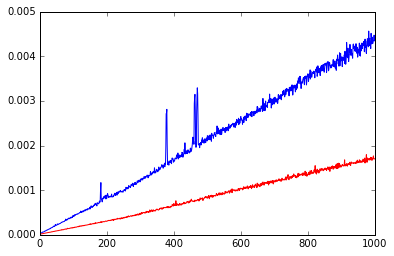
\includegraphics[scale=0.8]{./QuickSort/{pic/q7.png}}
    %\caption{}
\end{figure}



\chapter{Optimizing Program Performance}

\begin{enumerate}
    \item select an appropriate set of algorithms and data structures
    \item  write source code that the compiler can effectively optimize to turn into efficient executable code
    \item  divide a task into portions that can be computed in parallel, on some combination of multiple cores and multiple processors.
\end{enumerate}
명심할것. 두번째를 이해하기위해 컴파일러의 능력과 한계를 알아야한다. 최적화를 위하면서도 코드 가독성은 유지해야한다.


\section{Capabilities and Limitations of Optimizing Compilers}


컴파일러 최적화 명령어는 -0g -1g -2g ... 이 있다.


다음 두개의 코드가 있다고 생각해보자 
\begin{lstlisting}[style = CStyle]
void twiddle1(long *xp, long *yp)
{
*xp += *yp;
*xp += *yp;
}

void twiddle2(long *xp, long *yp)
{
*xp += 2* *yp;
}
\end{lstlisting}
twiddle1은 twiddle2로 최적화 될수있는가? 답은 아니 다. xp와 yp가 동일하다고 생각해보자. 그러면 명확할 것이다.


\begin{lstlisting}[style = CStyle]
long f();
long func1() {
return f() + f() + f() + f();
}

long func2() {
return 4*f();
}
\end{lstlisting}
func1 이 func2로 최적화 될 수 있다고 생각한다. 하지만 f에서 전역변수를 건든다고 생각해보자 4번 바뀔게 한번만 바뀌는 일이 될것이다.

컴파일러는 위험요소가 있을경우 최적화를 하지않는다.

\section{Eliminating Loop Inefficiencies}

\begin{lstlisting}[style = CStyle]
void combine1(vec_ptr v, data_t *dest)
 {
 long i;

 *dest = IDENT;
 for (i = 0; i < vec_length(v); i++) {
 data_t val;
 get_vec_element(v, i, &val);
 *dest = *dest OP val;
 }
 }

\end{lstlisting}

이게 어떻게 성능 개선이되는지 보자.

\begin{lstlisting}[style = CStyle]
void combine2(vec_ptr v, data_t *dest)
 {
 long i;
 long length = vec_length(v);

 *dest = IDENT;
 for (i = 0; i < length; i++) {
 data_t val;
 get_vec_element(v, i, &val);
 *dest = *dest OP val;
 }
 }
\end{lstlisting}


\begin{figure}[h!]
    \centering
    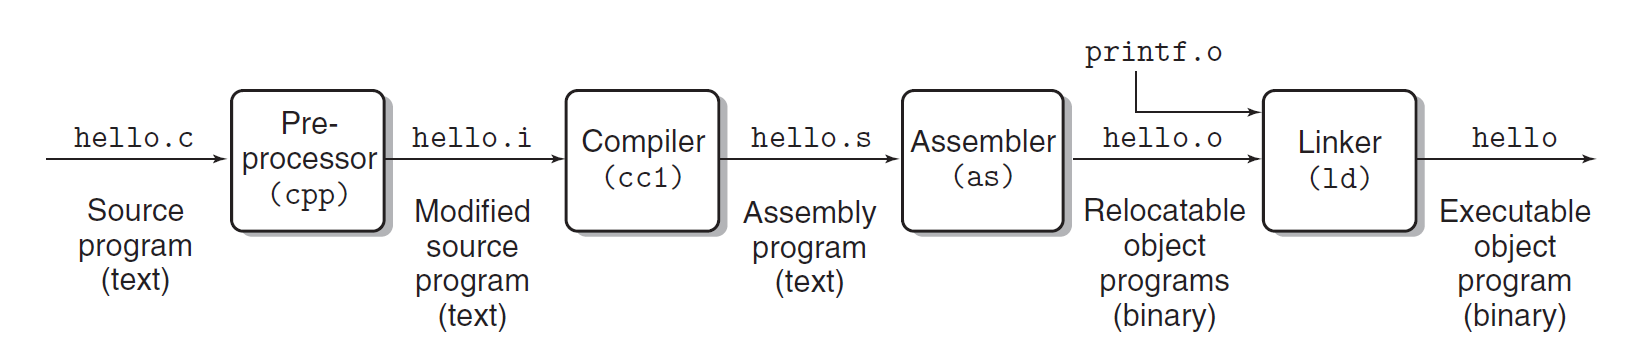
\includegraphics[scale=0.4]{pic/section5/pic1}
\end{figure}



\begin{lstlisting}[style = CStyle]
/* Convert string to lowercase: slow */
void lower1(char *s)
{
    long i;

    for (i = 0; i < strlen(s); i++)
        if (s[i] >= `A' && s[i] <= 'Z')
            s[i] -= ('A' - 'a');    
}

/* Convert string to lowercase: faster */
void lower2(char *s)
{
    long i;
    long len = strlen(s);

    for (i = 0; i < len; i++)
        if (s[i] >= `A' && s[i] <= 'Z')
            s[i] -= (`A' - 'a');
}

/* Sample implementation of library function strlen */
/* Compute length of string */
size_t strlen(const char *s)
{
    long length = 0;
    while (*s != '\0') {
        s++;
        length++;
    }
    return length;
}
\end{lstlisting}

\begin{figure}[h!]
    \centering
    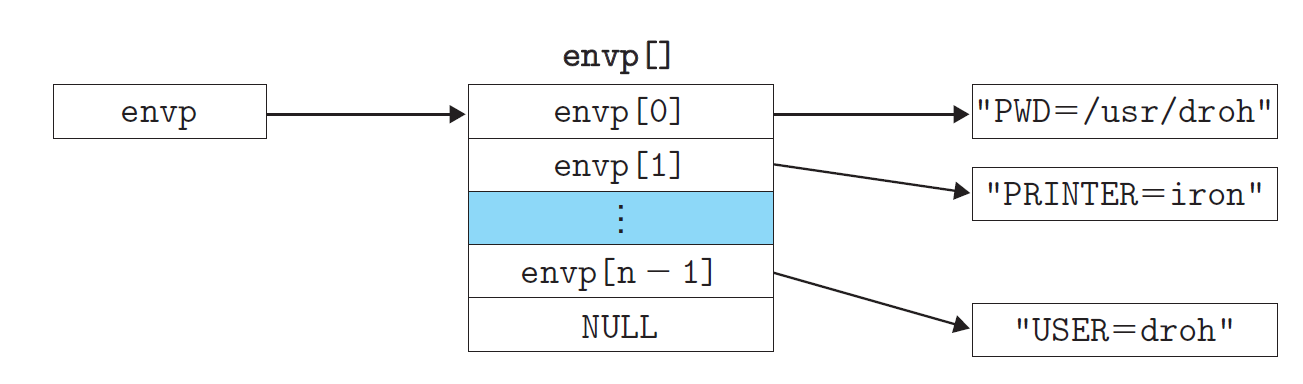
\includegraphics[scale=0.4]{pic/section5/pic2}
    \caption{lower 성능비교}
\end{figure}

시간복잡도 계산으로도 충분히 알 수 있다.
문자열 길이가 변하는게 아니라면 strlen을 반복문안에 넣는 짓은 하지말자.

\section{Reducing Procedure Calls}

\begin{lstlisting}[style = CStyle]
void combine3(vec_ptr v, data_t *dest)
{
    long i;
    long length = vec_length(v);
    data_t *data = get_vec_start(v);
    *dest = IDENT;
    for (i = 0; i < length; i++) {
    *dest = *dest OP data[i];
    }
}
\end{lstlisting}

대충 함수안에서 계속 함수를 쳐부르는 짓은 오버헤드와 불리는 함수안에서 처리하는 불필요한 작업으로 느려진다는 뜻.
근데 뒤에 더다룬다함


\begin{figure}[h!]
    \centering
    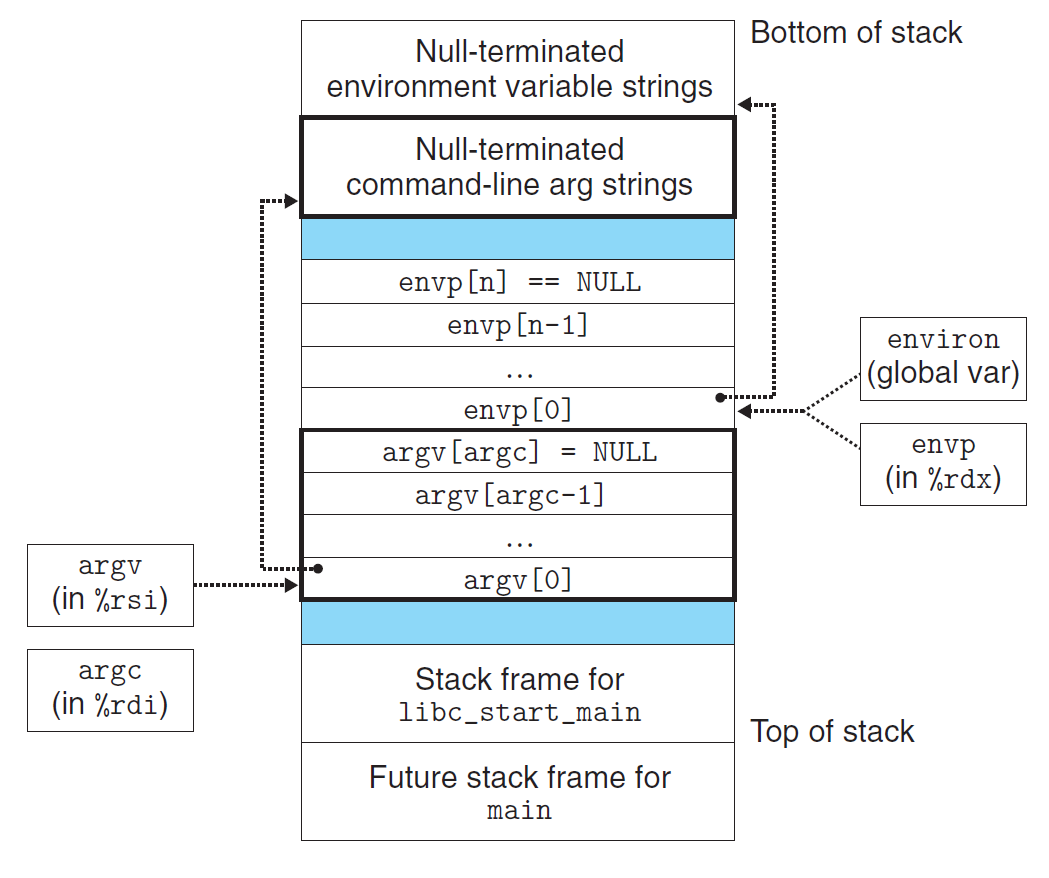
\includegraphics[scale=0.3]{pic/section5/pic3}
\end{figure}

\section{Eliminating Unneeded Memory References}

combine3에서 내부 루프는 포인터 dest가 메모리 참조를 계속하는 식이다.
다음 방식이 조금더 효율적이다.

\begin{lstlisting}[style = CStyle]
void combine4(vec_ptr v, data_t *dest)
 {
 long i;
 long length = vec_length(v);
 data_t *data = get_vec_start(v);
 data_t acc = IDENT;

for (i = 0; i < length; i++) {
 acc = acc OP data[i];
 }
 *dest = acc;
 }
\end{lstlisting}




\begin{figure}[h!]
    \centering
    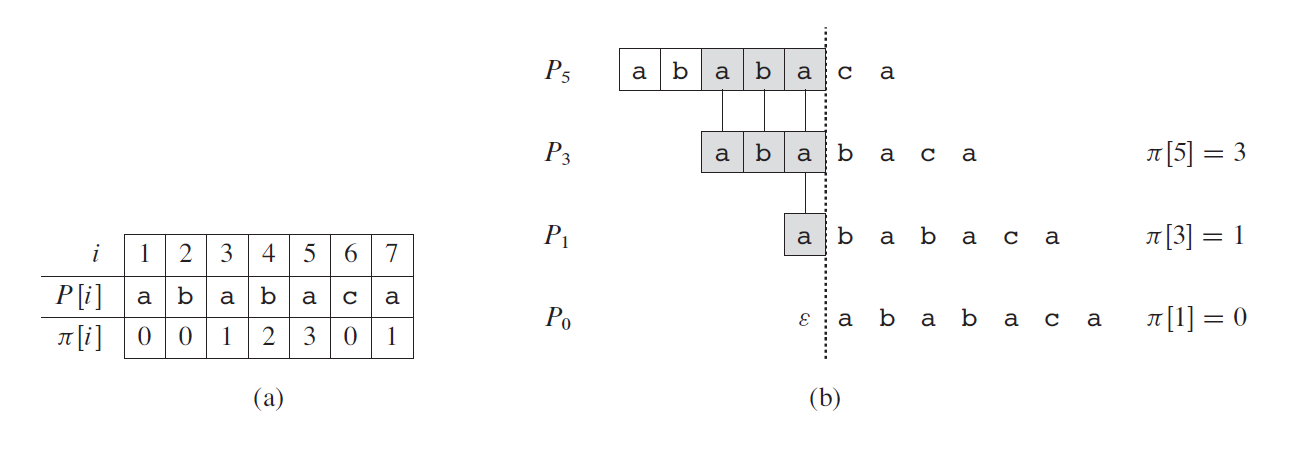
\includegraphics[scale=0.3]{pic/section5/pic4}
\end{figure}



\section{Understanding Modern Processors}

아몰랑


\section{Loop Unrolling}

while의 작동방식을 어셈블리로 한번보면 
if와  goto를 합쳐놓은 방식이다.
if는 단일 연산에비해느림 따라서
if검사를 적게 하게하면(=반복되는 횟수를 줄이면) 성능개선이 이루어진다.

\begin{lstlisting}[style = CStyle]
/* 2 x 1 loop unrolling */
void combine5(vec_ptr v, data_t *dest)
    {
    long i;
    long length = vec_length(v);
    long limit = length-1;
    data_t *data = get_vec_start(v);
    data_t acc = IDENT;

    /* Combine 2 elements at a time */
    for (i = 0; i < limit; i+=2) {
    acc = (acc OP data[i]) OP data[i+1];
    }

    /* Finish any remaining elements */
    for (; i < length; i++) {
    acc = acc OP data[i];
    }
    *dest = acc;
}
\end{lstlisting}


\begin{figure}[h!]
    \centering
    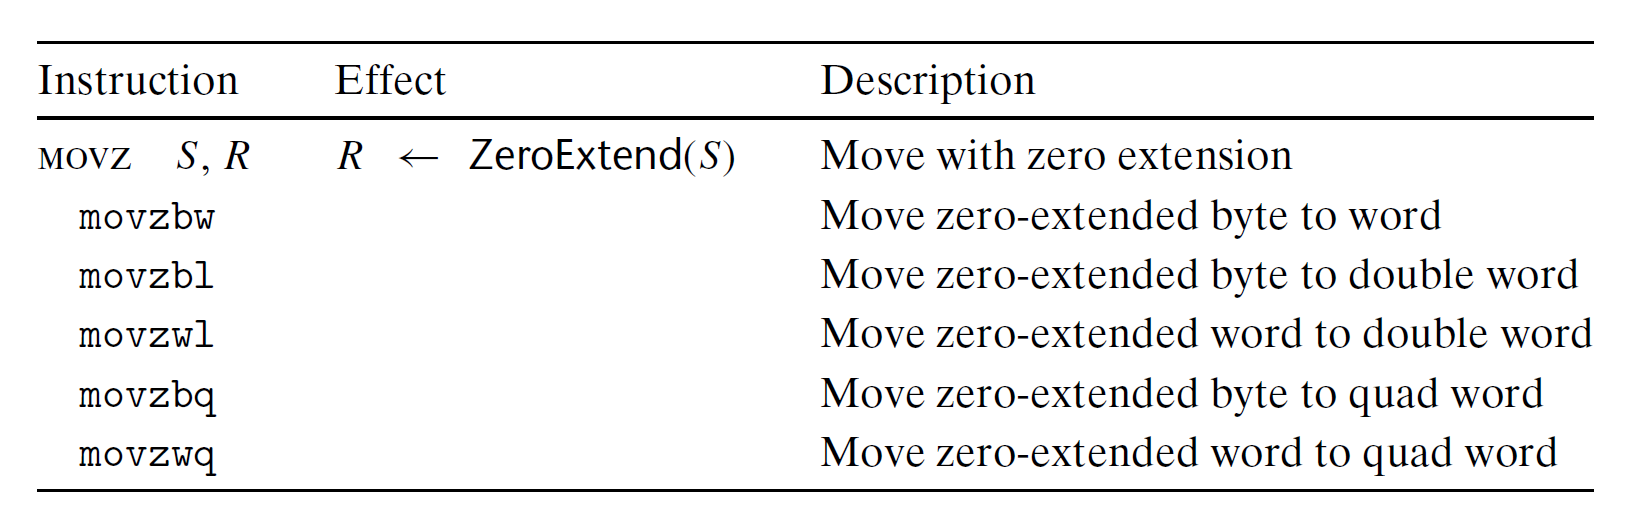
\includegraphics[scale=0.3]{pic/section5/pic5}
\end{figure}


\begin{figure}[h!]
    \centering
    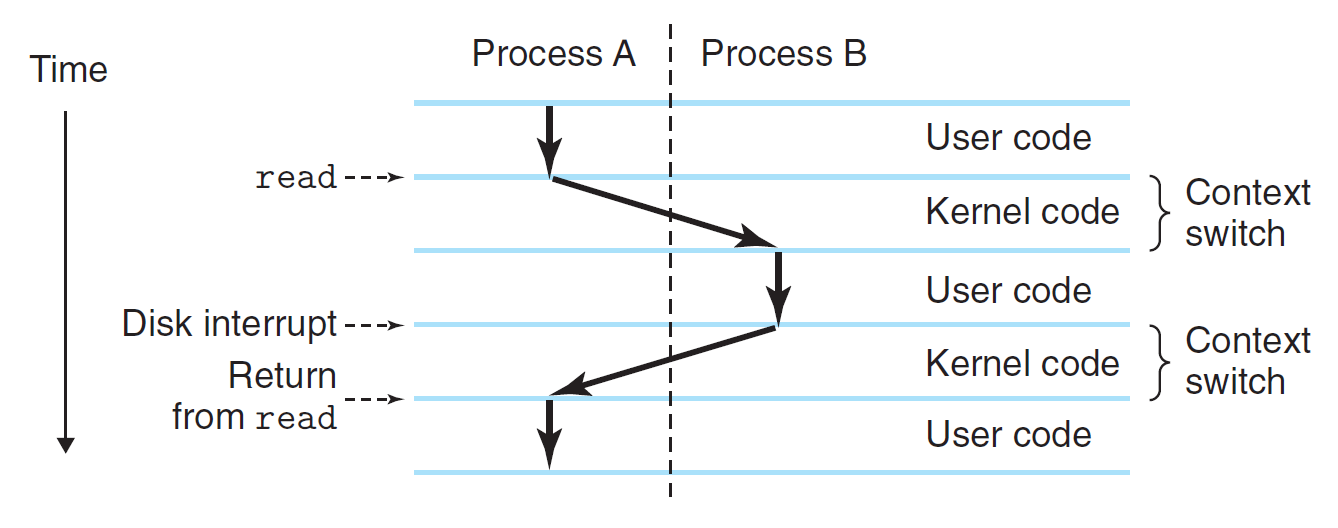
\includegraphics[scale=0.4]{pic/section5/pic6}
    \caption{ kx1 에따른 성능비교}
\end{figure}


이 생각을 할수있다.
루프풀기를 최대로하면 제일 좋은게아닌가?

여러단점이있다.

\url{http://z3moon.com/프로그래밍/loop_unrolling}

\url{https://en.wikipedia.org/wiki/Loop_unrolling}

\begin{enumerate}
    \item 코드 크기 증가
    \item 가독성 저해
    \item 함수호출이 있을 경우 캐시 미스율 향상
\end{enumerate}

연산이 복잡해질수록 인덱스의 계산과 if조건이 수행시간에 영향을 주지않는다.
for문 내부가 간단한 코드일때 가장 효과가 좋다.

\section{Enhancing Parallelism}

\subsubsection{Multiple Accumulators}
연산을 나눠서 계산하고 마지막에 합치는 방식

\begin{lstlisting}[style = CStyle]
/* 2 x 2 loop unrolling */
void combine6(vec_ptr v, data_t *dest)
{
    long i;
    long length = vec_length(v);
    long limit = length-1;
    data_t *data = get_vec_start(v);
    data_t acc0 = IDENT;
    data_t acc1 = IDENT;

    /* Combine 2 elements at a time */
    for (i = 0; i < limit; i+=2) {
    acc0 = acc0 OP data[i];
    acc1 = acc1 OP data[i+1];
    }

    /* Finish any remaining elements */
    for (; i < length; i++) {
    acc0 = acc0 OP data[i];
    }
    *dest = acc0 OP acc1;
}
\end{lstlisting}

\begin{figure}[h!]
    \centering
    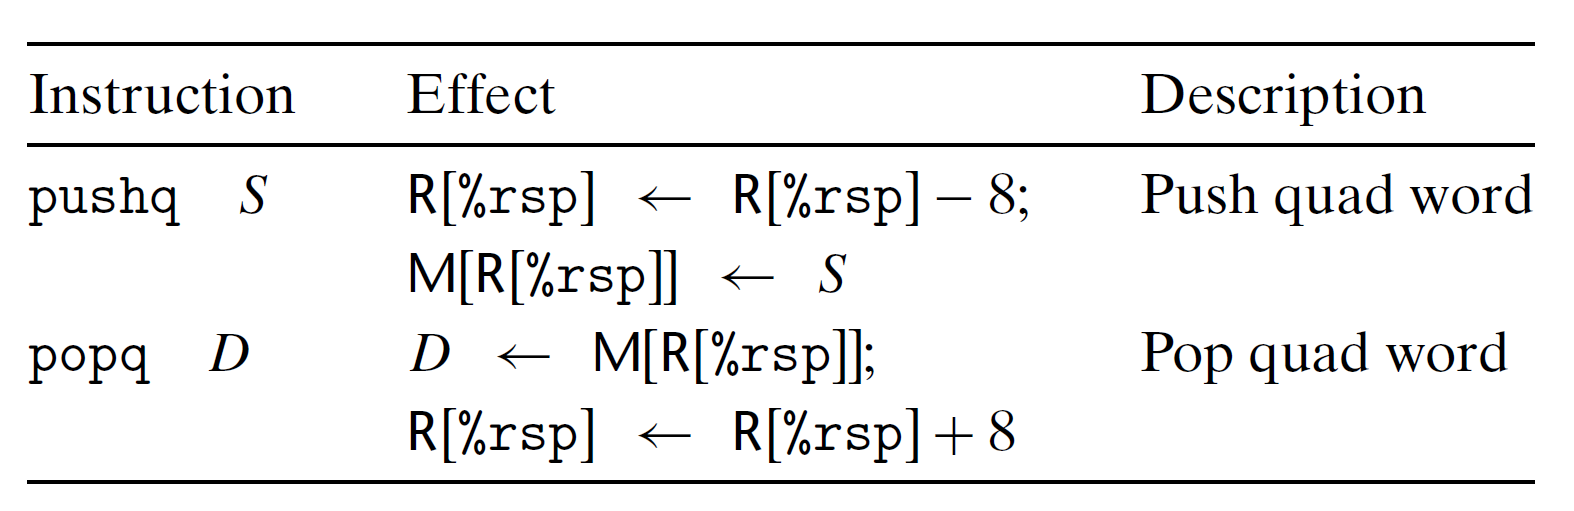
\includegraphics[scale=0.3]{pic/section5/pic7}
\end{figure}



\begin{figure}[h!]
    \centering
    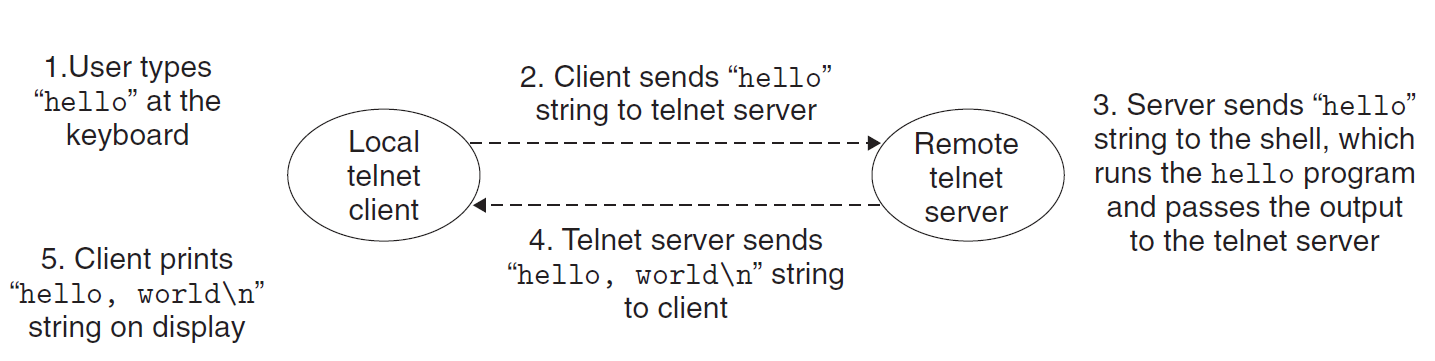
\includegraphics[scale=0.3]{pic/section5/pic8}
    \caption{kxk}
\end{figure}


\subsubsection{Reassociation Transformation}


\begin{lstlisting}[style = CStyle]
/* 2 x 1a loop unrolling */
void combine7(vec_ptr v, data_t *dest)
{
long i;
long length = vec_length(v);
long limit = length-1;
data_t *data = get_vec_start(v);
data_t acc = IDENT;

/* Combine 2 elements at a time */
for (i = 0; i < limit; i+=2) {
acc = acc OP (data[i] OP data[i+1]);
}

/* Finish any remaining elements */
for (; i < length; i++) {
acc = acc OP data[i];
}
*dest = acc;
}
\end{lstlisting}

combine5의 다음코드를


\begin{lstlisting}[style = CStyle]
    acc = (acc OP data[i]) OP data[i+1];
\end{lstlisting}


\begin{lstlisting}[style = CStyle]
    acc = acc OP (data[i] OP data[i+1]);
\end{lstlisting}
로 바꾼다.

\begin{figure}[h!]
    \centering
    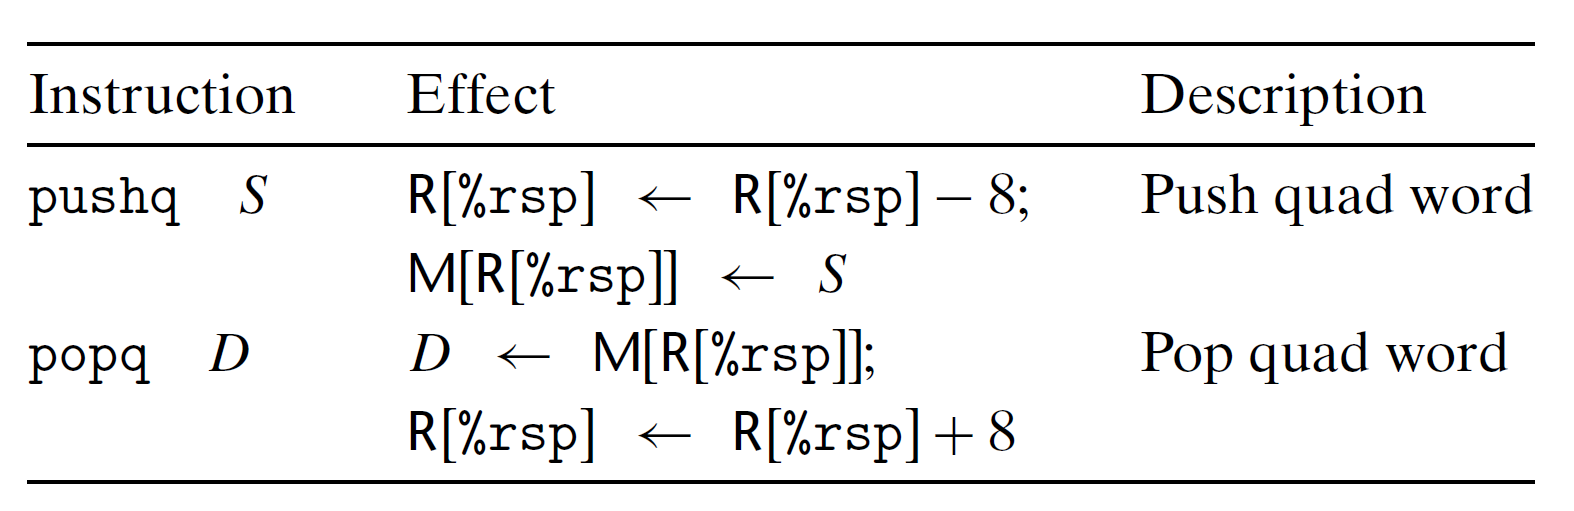
\includegraphics[scale=0.3]{pic/section5/pic7}
    \caption{}
\end{figure}



\begin{figure}[h!]
    \centering
    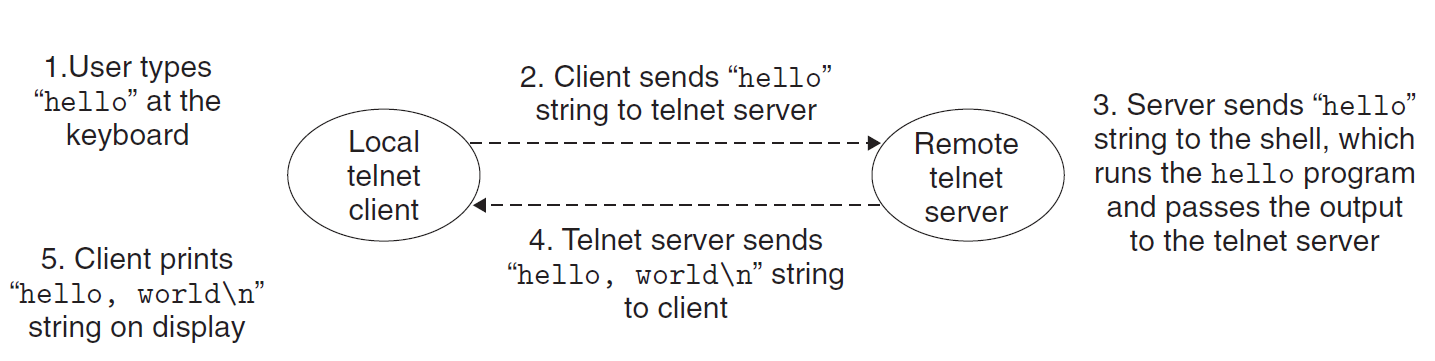
\includegraphics[scale=0.3]{pic/section5/pic8}
    \caption{}
\end{figure}



    %https://academic.naver.com/article.naver?doc_id=13986337

    %https://en.wikipedia.org/wiki/Pr%C3%BCfer_sequence

    %http://blog.daum.net/eternaljk/6176142

    %    https://www.math.uchicago.edu/~may/VIGRE/VIGRE2006/PAPERS/Casarotto.pdf

\end{document}